
%(BEGIN_QUESTION)
% Copyright 2006, Tony R. Kuphaldt, released under the Creative Commons Attribution License (v 1.0)
% This means you may do almost anything with this work of mine, so long as you give me proper credit

Calculate values for the following calibration table, for a transmitter measuring liquid level interface (specific gravities = 0.8 and 1.0), with a calibration tolerance of $\pm$ 1\% and a 4-20 mA output range.  Be sure to specify which port on the $\Delta$P transmitter to apply the calibration pressure:

$$\includegraphics[width=15.5cm]{i00310x01.eps}$$

% No blank lines allowed between lines of an \halign structure!
% I use comments (%) instead, so that TeX doesn't choke.

$$\vbox{\offinterlineskip
\halign{\strut
\vrule \quad\hfil # \ \hfil & 
\vrule \quad\hfil # \ \hfil & 
\vrule \quad\hfil # \ \hfil & 
\vrule \quad\hfil # \ \hfil & 
\vrule \quad\hfil # \ \hfil & 
\vrule \quad\hfil # \ \hfil \vrule \cr
\noalign{\hrule}
%
% First row
Interface & Percent of & $\Delta$ pressure & Output signal & Output signal & Output signal \cr
%
% Another row
level (ft) & span (\%) & sensed ("W.C) & ideal (mA) & min. (mA) & max. (mA) \cr
%
\noalign{\hrule}
%
% Another row
  & 0 &  &  &  &  \cr
%
\noalign{\hrule}
%
% Another row
  & 10 &  &  &  &  \cr
%
\noalign{\hrule}
%
% Another row
  & 25 &  &  &  &  \cr
%
\noalign{\hrule}
%
% Another row
  & 50 &  &  &  &  \cr
%
\noalign{\hrule}
%
% Another row
  & 75 &  &  &  &  \cr
%
\noalign{\hrule}
%
% Another row
  & 90 &  &  &  &  \cr
%
\noalign{\hrule}
%
% Another row
  & 100 &  &  &  &  \cr
%
\noalign{\hrule}
} % End of \halign 
}$$ % End of \vbox

Be sure to show all your mathematical work so that your instructor will be able to check the conceptual validity of your technique(s).  A good way to check to see if you're solving the problem correctly is to check that each and every one of your intermediate calculations (i.e. the results you get mid-way during the process to arrive at the final answer) has real physical meaning.  {\bf If you truly understand what you are doing, you will be able to identify the correct unit of measurement for every intermediate result and also be able to show where that number applies to the scenario at hand}.

\vskip 20pt \vbox{\hrule \hbox{\strut \vrule{} {\bf Suggestions for Socratic discussion} \vrule} \hrule}

\begin{itemize}
\item{} Demonstrate how to {\it estimate} numerical answers for this problem without using a calculator.
\item{} How will this level transmitter respond if the gas pressure inside this vessel were to increase?
\item{} How will this level transmitter respond if the gas pressure inside this vessel were to decrease?
\item{} How will this level transmitter respond if the overflow pipe were to be blocked off, so no light liquid could exit the vessel?
\item{} How will this level transmitter respond if the heavier fluid's density were to increase, yet the interface level remain the same?
\item{} How will this level transmitter respond if the lighter fluid's density were to increase, yet the interface level remain the same?
\end{itemize}

\underbar{file i00310}
%(END_QUESTION)





%(BEGIN_ANSWER)

{\bf Partial answer:}

% No blank lines allowed between lines of an \halign structure!
% I use comments (%) instead, so that TeX doesn't choke.

$$\vbox{\offinterlineskip
\halign{\strut
\vrule \quad\hfil # \ \hfil & 
\vrule \quad\hfil # \ \hfil & 
\vrule \quad\hfil # \ \hfil & 
\vrule \quad\hfil # \ \hfil & 
\vrule \quad\hfil # \ \hfil & 
\vrule \quad\hfil # \ \hfil \vrule \cr
\noalign{\hrule}
%
% First row
Interface & Percent of & $\Delta$ pressure & Output signal & Output signal & Output signal \cr
%
% Another row
level (ft) & span (\%) & sensed ("W.C) & ideal (mA) & min. (mA) & max. (mA) \cr
%
\noalign{\hrule}
%
% Another row
0 & 0 &  &  &  &  \cr
%
\noalign{\hrule}
%
% Another row
  & 10 &  &  &  & 5.76 \cr
%
\noalign{\hrule}
%
% Another row
  & 25 &  &  &  &  \cr
%
\noalign{\hrule}
%
% Another row
  & 50 &  & 12 &  &  \cr
%
\noalign{\hrule}
%
% Another row
4.5  & 75 &  &  &  &  \cr
%
\noalign{\hrule}
%
% Another row
  & 90 &  &  &  &  \cr
%
\noalign{\hrule}
%
% Another row
 & 100 & 43.2 (Low side) &  & 19.84 &  \cr
%
\noalign{\hrule}
} % End of \halign 
}$$ % End of \vbox

\vskip 10pt

Follow-up question: why do you suppose it is a good idea to keep the wet leg filled with a fluid with such a high specific gravity (1.2)?  Why not just let it flood with the lighter fluid (SG = 0.8) or even fill it with water (SG = 1.0)?

%(END_ANSWER)





%(BEGIN_NOTES)

\noindent
{\bf LRV condition}:

There will be 9 feet of light liquid sensed by the transmitter's ``H'' port and 10 feet of heavy liquid (SG = 1.2) sensed by the ``L'' port.  The differential pressure in the LRV interface condition will therefore be:

$$\hbox{DP}_{LRV} = \left(9 \hbox{ ft} \over 1 \right) \left(12 \hbox{ in} \over 1 \hbox{ ft}\right) \left(0.8 \hbox{ in water} \over 1 \hbox{ in liquid} \right) - \left(10 \hbox{ ft} \over 1 \right) \left(12 \hbox{ in} \over 1 \hbox{ ft}\right) \left(1.2 \hbox{ in water} \over 1 \hbox{ in liquid} \right) $$

$$\hbox{DP}_{LRV} = (86.4 \hbox{ "WC}) - (144 \hbox{ "WC}) = -57.6 \hbox{ "WC}$$

\vskip 10pt

\noindent
{\bf URV condition}:

There will be 6 feet of water-density liquid and 3 feet of light liquid sensed by the transmitter's ``H'' port and 10 feet of heavy liquid (SG = 1.2) sensed by the ``L'' port.  The differential pressure in the URV interface condition will therefore be:

$$\hbox{DP}_{URV} = \left(6 \hbox{ ft} \over 1 \right) \left(12 \hbox{ in} \over 1 \hbox{ ft}\right) + \left(3 \hbox{ ft} \over 1 \right) \left(12 \hbox{ in} \over 1 \hbox{ ft}\right) \left(0.8 \hbox{ in water} \over 1 \hbox{ in liquid} \right) - \left(10 \hbox{ ft} \over 1 \right) \left(12 \hbox{ in} \over 1 \hbox{ ft}\right) \left(1.2 \hbox{ in water} \over 1 \hbox{ in liquid} \right) $$

$$\hbox{DP}_{URV} = (72 \hbox{ "WC}) + (28.8 \hbox{ "WC}) - (144 \hbox{ "WC}) = -43.2 \hbox{ "WC}$$


% No blank lines allowed between lines of an \halign structure!
% I use comments (%) instead, so that TeX doesn't choke.

$$\vbox{\offinterlineskip
\halign{\strut
\vrule \quad\hfil # \ \hfil & 
\vrule \quad\hfil # \ \hfil & 
\vrule \quad\hfil # \ \hfil & 
\vrule \quad\hfil # \ \hfil & 
\vrule \quad\hfil # \ \hfil & 
\vrule \quad\hfil # \ \hfil \vrule \cr
\noalign{\hrule}
%
% First row
Interface & Percent of & $\Delta$ pressure & Output signal & Output signal & Output signal \cr
%
% Another row
level (ft) & span (\%) & sensed ("W.C) & ideal (mA) & min. (mA) & max. (mA) \cr
%
\noalign{\hrule}
%
% Another row
0 & 0 & 57.6 (Low side) & 4 & 3.84 & 4.16 \cr
%
\noalign{\hrule}
%
% Another row
0.6 & 10 & 56.16 (Low side) & 5.6 & 5.44 & 5.76 \cr
%
\noalign{\hrule}
%
% Another row
1.5 & 25 & 54 (Low side) & 8 & 7.84 & 8.16 \cr
%
\noalign{\hrule}
%
% Another row
3 & 50 & 50.4 (Low side) & 12 & 11.84 & 12.16 \cr
%
\noalign{\hrule}
%
% Another row
4.5  & 75 & 46.8 (Low side) & 16 & 15.84 & 16.16 \cr
%
\noalign{\hrule}
%
% Another row
5.4 & 90 & 44.64 (Low side) & 18.4 & 18.24 & 18.56 \cr
%
\noalign{\hrule}
%
% Another row
6 & 100 & 43.2 (Low side) & 20 & 19.84 & 20.16 \cr
%
\noalign{\hrule}
} % End of \halign 
}$$ % End of \vbox

It is good to keep the wet leg filled with a fluid heavier than {\it any} of the process components, just in case the interface level rises above the top of the wet leg.

\vskip 10pt

Note that in this situation, the ``low pressure'' side of the DP cell is {\it always} exposed to more pressure than the ``high pressure'' side!  At first this seems paradoxical, until you realize the terms ``high'' and ``low'' do not refer to absolute pressure, but rather to the {\it direction of influence} each port has over the transmitter's output.  Probably a better set of labels than ``high'' and ``low'' would be ``noninverting'' and ``inverting'' just like we use to describe differential amplifier inputs.

\vskip 10pt

The 3 foot horizontal dimension is extraneous information, included for the purpose of challenging students to identify whether or not information is relevant to solving a particular problem.

%INDEX% Measurement, interface level: calibration table

%(END_NOTES)


